\begin{enumerate}
	\item Pour une fonction du second degré $f(x) = ax^2+bx+c$, l'abscisse du sommet de la parabole
	est $x_S = -\dfrac{b}{2a}$. Ici $a = 1$ et $b = 2$, donc
	\[x_S = -\dfrac{2}{2 \times 1} = -1 \qquad\text{et}\qquad f(-1) = (-1)^2 + 2\times(-1) - 3 = 1 - 2 - 3 = -4.\]
	Le sommet de la parabole $\mathcal{P}$ a pour coordonnées $(-1 ; -4)$.

	\item
	\begin{enumerate}
		\item $g(-3) = (-3)^2 + (-3) - 6 = 9 - 3 - 6 = 0$ \quad et \quad $g(2) = 2^2 + 2 - 6 = 4 + 2 - 6 = 0$.

		Les réels $-3$ et $2$ sont donc racines de la fonction $g$.

		\item $g$ est une fonction du second degré de coefficient dominant $1 > 0$ : $g$ est positive à l'extérieur de ses racines et négative entre les
		deux.

		\begin{center}
			\begin{tikzpicture}
				\tkzTabInit[lgt=3.4,espcl=2.6]{$x$/1,$g(x)$/1}{$-\infty$,$-3$,$2$,$+\infty$}
				\tkzTabLine{,+,z,-,z,+,}
			\end{tikzpicture}
		\end{center}
	\end{enumerate}

	\item Pour tout réel $x$ :
	\[f(x) - h(x) = \left(x^2 + 2x - 3\right) - (x+3) = x^2 + 2x - 3 - x - 3 = x^2 + x - 6 = g(x).\]

	\item Étudier la position relative de deux courbes revient à étudier le signe de la différence
	$f(x) - h(x) = g(x)$, étudié à la question \textbf{2. b.}
	
Pour tout $x \in ]-3~;~2[$, $g(x) <0 \iff f(x)-h(x) <0 \iff f(x) < h(x)$.
Donc $\mathcal{P}$ est en dessous de $\mathcal{D}$ sur $]-3~;~2[$.
Et $\mathcal{P}$ est au-dessus de $\mathcal{D}$ sur $]-\infty~;~-3[ \,\cup\, ]2~;~+\infty[$.

	Les points d'intersection correspondent aux annulations de $g$, c'est-à-dire $x = -3$ et
	$x = 2$ : $h(-3) = 0$ et $h(2) = 5$.

Les deux courbes se coupent aux points de coordonnées $(-3~;~0)$ et $(2~;~5)$.
	\item
	\begin{center}
		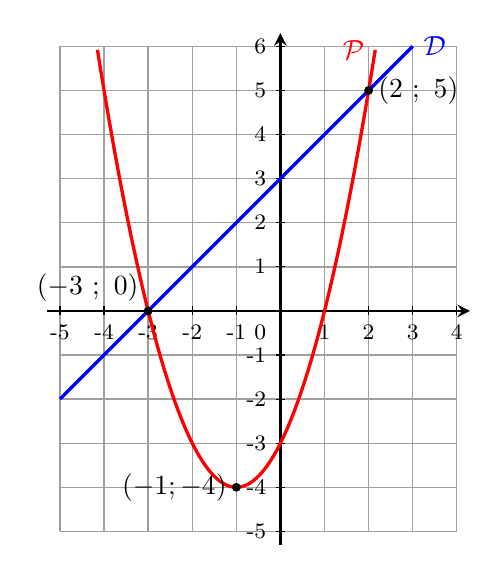
\begin{tikzpicture}[scale=0.8, x=7mm,y=7mm,>=stealth]
			\draw[step=1,gray!75,line width=0.5pt] (-5,-5) grid (4,6);
			\draw[->,line width=1pt] (-5.3,0) -- (4.3,0);
			\draw[->,line width=1pt] (0,-5.3) -- (0,6.3);
			\foreach \x in {-5,-4,-3,-2,-1,1,2,3,4} \draw (\x,2pt) -- (\x,-2pt) node[below] {\footnotesize \np{\x}};
			\foreach \y in {-5,-4,-3,-2,-1,1,2,3,4,5,6} \draw (2pt,\y) -- (-2pt,\y) node[left] {\footnotesize \np{\y}};
			\draw (-2pt,-2pt) node[below left]{\footnotesize 0};
			\draw[red,line width=1.2pt,domain=-4.15:2.15,samples=80]
			plot(\x,{(\x)^2+2*(\x)-3}) node[left,red]{$\mathcal{P}$};
			\draw[blue,line width=1.2pt] (-5,-2) -- (3,6) node[right,blue]{$\mathcal{D}$};
			\fill (-1,-4) circle(2pt) node[left]{$(-1;-4)$};
			\fill (-3,0) circle(2pt) node[above left]{$(-3~;~0)$};
			\fill (2,5) circle(2pt) node[right]{$(2~;~5)$};
		\end{tikzpicture}
	\end{center}
\end{enumerate}
